\documentclass[11pt,a4paper]{article}

% =========================================================
% HSLU Final Report --- DSPRO1 FS26 --- Team 8
% Project: Predicting Apartment Rental Prices in Switzerland
% =========================================================

% ---------- Encoding & Language ----------
\usepackage[T1]{fontenc}
\usepackage[utf8]{inputenc}
\usepackage[english]{babel}

% ---------- Typography ----------
\usepackage{lmodern}
\usepackage{microtype}
\usepackage{setspace}
\onehalfspacing

% ---------- Layout ----------
\usepackage[a4paper,margin=2.5cm]{geometry}
\setlength{\parindent}{0pt}
\setlength{\parskip}{0.6em}

% ---------- Colors ----------
\usepackage{xcolor}
\definecolor{hsluRed}{HTML}{E30613}
\definecolor{textGray}{HTML}{4F4F4F}
\definecolor{boxGray}{HTML}{F7F7F7}

% ---------- Graphics & Tables ----------
\usepackage{graphicx}
\usepackage{float}
\graphicspath{{fig/}{./}}
\usepackage{booktabs}
\usepackage{array}
\usepackage{tabularx}
\usepackage{multirow}
\usepackage{caption}
\captionsetup{font=small,labelfont=bf}

% ---------- Section formatting ----------
\usepackage{titlesec}
\titleformat{\section}{\Large\bfseries}{\thesection}{0.6em}{}
\titleformat{\subsection}{\normalsize\bfseries}{\thesubsection}{0.6em}{}
\titlespacing*{\section}{0pt}{1.0em}{0.4em}

% ---------- Hyperlinks ----------
\usepackage[hidelinks]{hyperref}

% ---------- References ----------
\usepackage[numbers]{natbib}

% ---------- Helper: figure placeholder when fig/<name>.png is missing ----------
\newcommand{\figplaceholder}[2]{%
\fbox{\parbox[c][#1][c]{0.78\linewidth}{\centering\textit{\textcolor{textGray}{#2}}}}%
}

% ---------- Helper: automatically load PNG if available ----------
\newcommand{\autofigure}[6]{%
\begin{figure}[H]
    \centering
    \IfFileExists{fig/#1}{%
        \includegraphics[width=#2]{fig/#1}%
    }{%
        \figplaceholder{#3}{#4}%
    }%
    \caption{#5}
    \label{#6}
\end{figure}
}

% ---------- Helper: draft note ----------
\newcommand{\draftnote}[1]{%
{\small\itshape\textcolor{textGray}{[Draft note: #1]}}%
}

\begin{document}

% =========================================================
% Title page
% =========================================================
\begin{titlepage}
\thispagestyle{empty}
\begin{center}


\includegraphics[width=0.20\textwidth]{hslu.jpg}

\vspace{0.45cm}

{\normalsize School of Computer Science and Information Technology\par}
{\normalsize Lucerne University of Applied Sciences and Arts (Switzerland)\par}

\vfill

{\fontsize{23}{28}\selectfont\bfseries Predicting Apartment\\Rental Prices in Switzerland\par}
\vspace{0.4cm}
{\fontsize{12}{15}\selectfont A Supervised Machine Learning Approach\\for the Swiss Cold-Rent Market\par}

\vfill

{\large DSPRO1 Final Report, Spring 2026 (FS26)\par}

\vspace{0.65cm}

\begin{minipage}{0.86\textwidth}
\centering
\small
presented to the School of Computer Science and Information Technology of\\
Lucerne University of Applied Sciences and Arts
\end{minipage}

\vfill

{\normalsize by\par}
\vspace{0.25cm}
{\Large Elias Martinelli \quad\textbar\quad Timo Schlumpf\par}
\vspace{0.2cm}
{\normalsize Team 8\par}

\vfill

{\normalsize Supervisor: Elena Nazarenko\par}
\vspace{0.35cm}
{\small Repository: \texttt{github.com/wadafacc/dspro1}\par}
\vspace{0.45cm}
{\normalsize Date: \today\par}

\end{center}
\end{titlepage}

\tableofcontents
\newpage

% =========================================================
\section*{Abstract}
\addcontentsline{toc}{section}{Abstract}
We build a supervised regression model that predicts the monthly cold rent of Swiss apartment listings from a self-scraped \texttt{rentumo.ch} snapshot ($\sim$4{,}500 listings, 13~April 2026), enriched with the Federal Register of Buildings and Dwellings (GWR) and several swisstopo layers (public-transport accessibility, elevation, solar suitability, hectare-grid population). On a fixed 80/20 train/eval split the strongest model is a LightGBM regressor with KNN-distance location features that reaches an evaluation RMSE of 393~CHF (R$^2$\,=\,0.751), reducing the mean-prediction baseline of 847~CHF by more than 50\%. A regularised 4-feature variant and a separate ``wide'' pipeline that almost doubles the training set are kept as alternative artefacts. A Streamlit demo app (\texttt{src/app.py}) exposes the trained pipeline via address lookup against the official GeoAdmin SearchServer. The original hypothesis, namely that a tree-based model would outperform a linear model on this task, is clearly accepted; the dominant remaining error source is luxury attributes (view, floor, finish) that the current tabular features do not capture and that should be extracted from the listing text in future work.

\newpage

% =========================================================
\section{Introduction}
\label{sec:introduction}

Apartment rents in Switzerland differ strongly by location, building type, and apartment characteristics. For someone comparing a listing such as ``CHF 2'400 per month, 3~rooms, 80\,m$^2$, Zurich'', it is difficult to judge whether the advertised price is reasonable. Public rent indicators are useful for understanding general market trends, but they do not give a concrete estimate for one specific apartment.

This project builds a supervised regression model for predicting the monthly cold rent (\emph{Kaltmiete}, in CHF) of individual Swiss apartment listings. The underlying dataset is \emph{not} a ready-made benchmark: we collected it ourselves by writing a custom scraper for \texttt{rentumo.ch}~\citep{rentumo}, a Swiss rental aggregator, and enriched the resulting listings with official Swiss open-register data from GWR and swisstopo. The task is treated as a tabular regression problem. Each apartment is described by structural features such as living area, number of rooms and year of construction, as well as location-based features such as coordinates, public-transport accessibility, elevation, population density and solar suitability. The target variable is the listed cold rent.

\paragraph{Research question and hypothesis.}
The main question is whether listing data, combined with Swiss open-register data from GWR and swisstopo, contains enough information to estimate apartment rents in a useful way. Based on the project proposal and the mid-term presentation, we formulated the following hypothesis:

\begin{quote}\itshape
``Location-related variables combined with structural apartment features contain sufficient signal to predict monthly rental prices in Switzerland with practically useful accuracy, and a Tree based model will outperform a Linear Regression model in doing so.''
\end{quote}

We test this hypothesis with several levels of model complexity: a simple baseline that ignores all features, a linear Ridge model as an interpretable benchmark, and a family of tree-based models including RandomForest, GradientBoosting, XGBoost, LightGBM, and a Stacking ensemble. The hypothesis is therefore phrased at the model-\emph{family} level rather than tying it to one specific algorithm, which reflects how the experimental design actually unfolded across the project.

\paragraph{Stakeholders and intended use.}
The most important users of such a model are tenants who want a first indication of whether an advertised rent is fair. Landlords and property managers may also benefit from a market-based reference value. The model should be understood as a decision-support tool. It is \emph{not} a legally binding rent assessment and does not replace formal rent reviews under Swiss tenancy law (OR Art.~269\,ff.). A simple Streamlit demo (\texttt{src/app.py}) exposes the trained \texttt{RentPredictor} interactively, so a non-technical user can enter a few apartment characteristics and immediately receive an estimate.

\paragraph{Report structure.}
The report is structured as follows. Section~\ref{sec:sota} gives an overview of related work in real-estate price prediction. Section~\ref{sec:data} describes the data sources, the enrichment process and the main quality checks. Section~\ref{sec:methods} explains the modelling pipeline, evaluation strategy and feature engineering. Section~\ref{sec:results} presents the results, including model comparison, residual diagnostics and error analysis. Section~\ref{sec:conclusions} closes with the main conclusions, limitations and possible next steps.

% =========================================================
\section{State of the Art}
\label{sec:sota}

Real-estate and rental-price prediction has been studied for a long time in both economics and machine learning. The traditional approach is \emph{hedonic pricing}: prices are modelled as a function of structural and location-related characteristics, often using linear regression. This idea goes back to Rosen~\citep{rosen1974hedonic}. Hedonic models are still widely used, especially by statistical offices, but they require strong assumptions about the functional form and can struggle with complex non-linear effects.

Modern machine-learning approaches use more flexible models instead of manually specifying all relationships. Tree-based ensembles such as RandomForest~\citep{breiman2001randomforest} and gradient boosting~\citep{friedman2001gbm} are particularly well suited for tabular regression. They can capture non-linear interactions, handle features with different scales and usually require only limited preprocessing. Optimised implementations such as XGBoost~\citep{chen2016xgboost} and LightGBM~\citep{ke2017lightgbm} add efficient training and regularisation, and often perform strongly on tabular benchmarks~\citep{shwartz2022tabular}.

Because rent estimates may influence real decisions, interpretability is important. SHAP values provide feature-attribution explanations for individual predictions and are commonly used together with tree-based models~\citep{lundberg2017shap}. For documenting the dataset and model, we follow the ideas of \emph{Datasheets for Datasets}~\citep{gebru2021datasheets} and \emph{Model Cards}~\citep{mitchell2019modelcards}.

For the Swiss housing market specifically, two public data sources are critical: the Federal Register of Buildings and Dwellings (GWR), maintained by the Federal Statistical Office (BFS)~\citep{bfsGwr}, and the swisstopo geo-services exposed through GeoAdmin~\citep{geoAdminApi}. The GWR provides per-building attributes (construction year, number of dwellings, building footprint) indexed by EGID, while swisstopo provides geo-layer attributes such as public-transport accessibility~\citep{areOevKlassen}, solar-suitability classes from the Federal Office of Energy (BFE)~\citep{bfeSolar}, and the BFS population-by-hectare grid~\citep{bfsPopulation}.

% =========================================================
\section{Data}
\label{sec:data}

\subsection{Sources and Collection}
The primary dataset, \emph{Rentumo Rental Listings Switzerland v1.0}, was collected from \texttt{rentumo.ch} in a single scrape on 13~April 2026. The scraper identified 25\,002 entries on the platform, of which 9\,994 listings could be extracted successfully. Many of the remaining pages were empty or non-functional placeholder pages, which appears to be a characteristic of the platform rather than an error in the scraper.

The scraper is implemented as a custom Rust library, \texttt{ScrapeGoat}, and operates in two sequential phases.

\paragraph{Phase 1: Listing index pages.}
The scraper issues requests to 750 paginated listing pages of the form \texttt{rentumo.ch/mietobjekte?types=apartment\&page=\{1..750\}}. Each page is parsed with CSS selectors targeting the \texttt{\#listings} container, from which per-listing elements yield the number of rooms, the living area in square metres, the cold rent, and a unique URL slug (e.g.\ \texttt{/inserate/<slug>}). Listings for which any of these four fields cannot be parsed are silently dropped at this stage. Successfully extracted records are written to the \texttt{listings} table in the PostgreSQL database with an \texttt{ON CONFLICT (slug) DO NOTHING} guard, making the phase idempotent and safe to re-run.

\paragraph{Phase 2: Detail pages.}
All slugs stored in \texttt{listings} are retrieved from the database and used to construct individual detail URLs (\texttt{rentumo.ch/inserate/<slug>}). Each detail page is parsed to extract additional fields: the full address, the cold rent as confirmed on the detail page, the living area, the number of rooms, the auxiliary costs (\emph{Nebenkosten}), the security deposit (\emph{Kaution}), a free-text description from the JSON-LD \emph{Apartment} schema block, and the earliest available move-in date (\emph{Datum verfügbar}). These are written to a separate \texttt{listing\_details} table with \texttt{ON CONFLICT (listing\_id) DO UPDATE}, allowing the phase to be resumed or repeated without data loss.

\paragraph{Concurrency and politeness.}
Both phases are managed by a custom task orchestrator (\texttt{Mgt}) that maintains a fixed pool of up to 10 concurrent in-flight HTTP requests. A channel-based feedback loop ensures that a new request is dispatched only when an existing one completes, bounding peak load on the server. Each request carries a randomly sampled \texttt{User-Agent} header drawn from a pre-loaded list, and optional HTTP proxies can be configured via a plain-text file to distribute outbound traffic across multiple IP addresses.

\paragraph{Platform selection.}
We also considered \texttt{comparis.ch} as a possible data source, but decided not to use it. Comparis confirmed in writing that automated extraction would require formal authorisation and that access would likely be limited to around 300 records, which would not be sufficient for this modelling task. Rentumo was contacted by email before the scrape, but no response was received. The data is used only for the non-commercial academic purpose of the DSPRO1 module.

\subsection{Enrichment}
The scraped listings contain the address and a small set of structural attributes, including \texttt{area\_sqm}, \texttt{rooms}, \texttt{price\_cold} and \texttt{auxiliary\_costs}. To make the dataset more useful for modelling, we enrich these listings in two steps:

\begin{enumerate}
    \item \textbf{GWR (BFS).} Each listing address is geocoded and resolved to a building identifier (EGID) via the GeoAdmin SearchServer. Building-level attributes (\texttt{gbauj} / construction year, \texttt{ganzwhg} / number of dwellings, \texttt{garea} / footprint area) are then queried from the GWR record.
    \item \textbf{swisstopo / GeoAdmin.} Using the LV95 coordinates (\texttt{lv95\_east}, \texttt{lv95\_north}), per-point attributes are queried from public layers: elevation (\texttt{elevation\_m}, height service), public-transport accessibility class (\texttt{oev\_score}, layer \texttt{ch.are.erreichbarkeit-oev}), solar suitability class 1--5 (\texttt{solar\_class}, layer \texttt{ch.bfe.solarenergie-eignung-daecher}), and the population of the nearest hectare cell (\texttt{population}, BFS Volkszählung).
\end{enumerate}

\subsection{Storage and Schema}
The raw and enriched data are stored in a PostgreSQL database on Neon Console. The relevant information is distributed across three tables: \texttt{listings} for the listing index, \texttt{listing\_details} for the extracted apartment attributes, and \texttt{swisstopo\_details} for the enriched geo-layer features. For modelling, these tables are joined into a flat file, \texttt{model.csv}, while requiring all mandatory columns to be present. After filtering and joining, the final modelling dataset contains approximately 4\,500 rows with 12 columns: 11 predictors and \texttt{price\_cold} as the target variable.

\autofigure
{geo_price_map.png}
{0.85\linewidth}
{5.5cm}
{Geographic distribution of the 4'500 modelling-set apartments across Switzerland, colored by cold rent. Urban centres (Zurich, Geneva, Basel) are clearly visible and overrepresented.}
{Geographic distribution of listings colored by cold rent.}
{fig:geo}

\subsection{Quality Assessment}
\begin{itemize}
    \item \textbf{Completeness.} Listings missing any of \texttt{address}, \texttt{price\_cold}, \texttt{area\_sqm}, or \texttt{rooms} are removed entirely. Listings marked ``Preis auf Anfrage'' are also removed. Of the 9\,994 scraped listings, approximately 4\,500 remain after the mandatory-field filter and the GWR/swisstopo join (cumulative loss is diagnosed in \texttt{final\_records.ipynb}).
    \item \textbf{Accuracy.} An explicit outlier filter (\texttt{area\_sqm}\,$\geq$\,10, \texttt{price\_cold}\,$\geq$\,300) removes implausible listings. An \texttt{IsolationForest} diagnostic (Notebook Chapter~22.9) surfaces additional candidates for manual review.
    \item \textbf{Consistency.} Cantons are normalised to ISO~3166-2:CH (\texttt{ZH}, \texttt{BE}, $\ldots$). The construction year is stored as a four-digit integer; missing GWR values are median-imputed.
    \item \textbf{Timeliness.} The dataset is a single point-in-time snapshot from 13 April 2026. Temporal price changes after that date are not reflected; time-series modelling is explicitly out of scope.
\end{itemize}

\autofigure
{price_distribution.png}
{0.78\linewidth}
{4.5cm}
{Histogram of monthly cold rent across the 4'500 modelling-set apartments. A strong right-skew is visible, with a long tail towards expensive apartments.}
{Distribution of the target variable \texttt{price\_cold}. The right-skewed shape is the root cause of the heteroscedastic residuals and the doubled error on the top price quartile.}
{fig:price-dist}

\autofigure
{feature_correlation.png}
{0.85\linewidth}
{5cm}
{Pearson correlation heatmap of the most important features with the target \texttt{price\_cold}. Only the top correlations with the target are shown, sorted in descending order.}
{Pearson correlation heatmap of the most important predictors with the target \texttt{price\_cold} (Notebook Chapter~4). The strongest single positive correlation is with \texttt{area} ($r\approx 0.74$), followed by the KNN-price features and the LV95 \texttt{east} coordinate. The heatmap intentionally lists the strongest correlations at the top so a reader can scan from top to bottom. \texttt{rooms} correlates strongly with \texttt{area} but only moderately with the target on its own, which is the empirical justification for engineering the \texttt{area\_per\_room} feature in Section~\ref{sec:methods}.}
{fig:feature-corr}

\subsection{Legal and Ethical Considerations}
No personal data is collected. Landlord names and contact details are explicitly excluded by the scraper. Only the address is retained and is used solely for geocoding and building-level enrichment. The project does not process any special-category data defined under the revised Swiss Federal Act on Data Protection (nFADP). The dataset is used exclusively for academic purposes and is not redistributed.

% =========================================================
\section{Methods}
\label{sec:methods}

\subsection{Pipeline Overview}
The modelling pipeline is implemented in \texttt{src/notebooks/model\_v3\_clean.ipynb}. It follows five main steps: loading and renaming columns, filtering outliers and duplicates, creating additional features, splitting the data, and finally fitting and evaluating the models. The final end-to-end logic is wrapped in a \texttt{RentPredictor} Python class (Notebook Chapter~24.2), which can be saved with \texttt{joblib} and loaded again for inference in the Streamlit demo app (\texttt{src/app.py}).

\subsection{Train/Eval/Test Split}
We use a fixed random seed (\texttt{random\_state=42}) to make the split reproducible. The main experiments use an 80\% training set and a 20\% evaluation set. For the final hold-out check (Notebook Chapter~24.6), we additionally use a 60/20/20 train/validation/test split. The evaluation and test sets are not used for model fitting. A Kolmogorov-Smirnov test (Chapter~22.13) is used to check that the random split does not introduce a strong distribution shift between training and evaluation data.

\subsection{Feature Engineering}
In addition to the raw features, three engineered features are added (Chapter~6):
\texttt{building\_age = REFERENCE\_YEAR - year\_built},
\texttt{area\_per\_room = area / rooms} using safe division, and
\texttt{land\_area\_per\_apartment = garea / ganzwhg}.
Two further feature groups are created using only \texttt{train\_df}, so that information from the evaluation set does not leak into training:

\begin{itemize}
    \item \textbf{Geo-clusters.} \texttt{KMeans} on standardised LV95 coordinates produces a discrete \texttt{geo\_cluster} feature (Chapter~21). The number of clusters is tuned on Eval RMSE.
    \item \textbf{KNN-distance features.} For each apartment, the median price of its 10 nearest neighbours in coordinate space (\texttt{knn\_price\_median}) and the corresponding mean (\texttt{knn\_price\_mean}) are added (Chapter~23.12). The nearest-neighbour index is fit on training data only; eval points query against the training index.
\end{itemize}

\autofigure
{geo_clusters.png}
{0.78\linewidth}
{5cm}
{Visualisation of the KMeans geo-clusters fitted on \texttt{train\_df} only. Each colour corresponds to one \texttt{geo\_cluster} category that is consumed by the tree models as a discrete feature.}
{KMeans geo-clusters used as a categorical location feature (Notebook Chapter~21.4). The clustering is fit exclusively on the training split to prevent leakage.}
{fig:geo-clusters}

\subsection{Models}
We compare six model families on the same data split. Where necessary, the models are wrapped in an \texttt{sklearn.Pipeline}. The comparison includes a \textbf{DummyRegressor} as a lower bound, a \textbf{Ridge} model with scaling as a simple linear benchmark, and four tree-based approaches: \textbf{RandomForestRegressor}, \textbf{GradientBoostingRegressor}, \textbf{XGBoost} and \textbf{LightGBM}. In Chapter~23.2, we also add a \textbf{StackingRegressor} with a Ridge meta-learner over the strongest tree-based models.

Hyperparameters are tuned with \texttt{RandomizedSearchCV} (Chapter~22.3) and the faster \texttt{HalvingRandomSearchCV} (Chapter~23.10). To avoid scikit-learn's nested-parallelism trap, the inner estimator is set to \texttt{n\_jobs=1} while only the outer search uses \texttt{n\_jobs=-1}.

\subsection{Experimental Features and Testing Milestones}
The pipeline was not designed in a single shot. Instead, it grew along a series of \emph{experimental milestones}, where the outcome of one milestone informed the design of the next. We treated each new feature, each new model and each new diagnostic as an experiment with a defined success criterion (evaluation RMSE compared to the previous milestone, plus a stability check on CV-RMSE) before it was accepted into the main pipeline. The notebook reflects this milestone-driven structure directly:

\begin{itemize}
    \item \textbf{M1 — Baselines (Chapters~1--12).} Establish the modelling problem, fix the split, run a \texttt{DummyRegressor} and a Ridge baseline, and confirm that a small set of tree-based models clearly beats both. This milestone defines the lower bound everything else must beat.
    \item \textbf{M2 — Geo features (Chapter~21).} Add KMeans \texttt{geo\_cluster} and explore DBSCAN as a diagnostic. The KMeans cluster is kept because it materially improves evaluation RMSE for the linear model and does not hurt the trees.
    \item \textbf{M3 — Diagnostics and tuning (Chapter~22).} Introduce \texttt{IsolationForest}-based outlier review, learning curves, log-target experiments, RFECV, drift checks and bias-per-cluster analysis. Most of these are experimental probes: only those that survive the milestone criterion (e.g.\ tuned LightGBM, drift confirmation) propagate forward.
    \item \textbf{M4 — Stacking, PDPs, KNN-features (Chapter~23).} The decisive milestone: \texttt{knn\_price\_median} and \texttt{knn\_price\_mean} reduce LightGBM's eval RMSE from 399 to 393~CHF and lift R$^2$ to 0.751, so they are promoted to the main feature set. PDPs and bootstrap CIs confirm the new model is also stable.
    \item \textbf{M5 — End-to-end and hold-out (Chapter~24).} Wrap the winning pipeline in a \texttt{RentPredictor} class, write the model card and datasheet, and verify on a strictly untouched 20\% test split that the chosen model has not overfit to the evaluation split.
    \item \textbf{M6 — Regularisation and wide pipeline (Chapters~27--28).} Two follow-up experiments aimed at the residual overfit gap: a regularised LightGBM on three reduced feature sets, and a \emph{wide} pipeline trained on $\sim$9.5k rows with only four features. The wide pipeline is kept as an alternative deliverable because it almost doubles the available training data.
\end{itemize}

Features that did not clear their milestone criterion (log-target inverse transform, DBSCAN cluster as a model feature, several stacking configurations) are retained in the notebook for transparency, but they are explicitly \emph{not} part of the final pipeline.

\subsection{Evaluation Metrics}
As defined in the project proposal, the main metrics are MAE, RMSE and R$^2$. RMSE is calculated as \texttt{np.sqrt(mean\_squared\_error(...))}, which keeps the code compatible across scikit-learn versions. The notebook also reports MedAE as a more robust error metric, the standard deviation of CV-RMSE across folds as a stability indicator, and bootstrap 95\% confidence intervals for RMSE on the evaluation set (Chapter~23.5). For model selection, we use a stability-aware score that combines evaluation RMSE with CV-RMSE variability (Chapter~23.9), so that a model is not chosen only because of one favourable split.

% =========================================================
\section{Results}
\label{sec:results}

\subsection{Baseline}
The baseline used in the mid-term presentation was a \texttt{DummyRegressor} with a mean-prediction strategy. It achieved MAE\,=\,612 CHF, RMSE\,=\,847 CHF and R$^2$\,=\,0.00. This gives a simple lower bound: a useful model must clearly perform better than predicting the same rent for every apartment.

\subsection{Model Comparison}
Table~\ref{tab:models} summarises the main results for the model comparison on the \texttt{FEATURES\_ENGINEERED} feature set (Notebook Chapter~10).

\begin{table}[h]
\centering
\small
\caption{Model comparison on the engineered feature set (Notebook Chapter~10c). RMSE values are in CHF on the held-out evaluation split.}
\label{tab:models}
\begin{tabular}{lrrrrl}
\toprule
Model & RMSE Train & RMSE Eval & R$^2$ Eval & Overfit Gap & Diagnosis \\
\midrule
LightGBM         & 150  & \textbf{399} & \textbf{0.744} & 249 & Possible overfit \\
XGBoost          & 122  & 421 & 0.715 & 299 & Possible overfit \\
GradientBoosting & 365  & 425 & 0.710 &  60 & Good generalisation \\
RandomForest     & 199  & 425 & 0.710 & 226 & Possible overfit \\
Ridge (scaled)   & 539  & 560 & 0.495 &  21 & Weak / underfit \\
Dummy (median)   & 737  & 799 & $-0.03$ & 62 & Baseline \\
\bottomrule
\end{tabular}
\end{table}

\autofigure
{rmse_train_eval.png}
{0.85\linewidth}
{4.5cm}
{Bar plot: RMSE Train vs.\ RMSE Eval per model.}
{Train vs.\ Eval RMSE per model. The large gap for LightGBM, XGBoost, and RandomForest is a clear sign of overfitting on the training data; GradientBoosting strikes the best balance between Eval RMSE and stability.}
{fig:rmse-bars}

The best single model according to evaluation RMSE is \emph{LightGBM}, with an RMSE of 399 CHF. After adding the KNN-distance features, LightGBM improves slightly further to \textbf{RMSE Eval\,=\,393 CHF and R$^2$\,=\,0.751} (Notebook Chapter~23.17, consolidated comparison). Compared with the mid-term baseline, this reduces RMSE by more than 50\%.

\paragraph{Hypothesis test.}
The project hypothesis was that a tree-based model would outperform a linear regression model on this task. The results support this hypothesis clearly. Ridge reaches an evaluation RMSE of 560~CHF, while \emph{every} tree-based model in the comparison achieves 425~CHF or better; the strongest of them, LightGBM with KNN-distance features, reaches 393~CHF. The difference between the linear and the tree-based family is therefore substantially larger than the differences between individual tree-based models, which is the reason the hypothesis is phrased at the family level. We accept the hypothesis.

\autofigure
{bootstrap_ci.png}
{0.85\linewidth}
{4.5cm}
{Forest plot of bootstrap 95\% confidence intervals for evaluation RMSE per model (Notebook Chapter~23.5). Overlapping intervals indicate model differences that are not statistically significant.}
{Bootstrap confidence intervals for evaluation RMSE per model. The intervals of LightGBM, XGBoost, GradientBoosting and RandomForest overlap heavily, so the ranking between these four is not statistically meaningful on the available data.}
{fig:bootstrap-ci}

\autofigure
{learning_curve.png}
{0.85\linewidth}
{4.5cm}
{Learning curve for the chosen LightGBM model showing train and CV RMSE as a function of the training-set size (Notebook Chapter~22.5).}
{Learning curve for the chosen LightGBM model (Notebook Chapter~22.5). The training RMSE stays low across all training-set sizes while the validation RMSE converges to roughly 400~CHF. The remaining gap is the visible signature of overfitting on the engineered feature set — it shrinks but does not close as more data is added, which is consistent with the finding in Section~\ref{sec:wide} that adding more data alone (without the engineered features) does not improve evaluation performance.}
{fig:learning-curve}

\subsection{Actual vs.\ Predicted and Residuals}

\autofigure
{actual_vs_predicted.png}
{0.88\linewidth}
{4.5cm}
{Actual vs.\ predicted plot missing. Expected file: \texttt{fig/actual\_vs\_predicted.png}.}
{Actual vs.\ predicted cold rent on the evaluation set for the best LightGBM model. Points clustering near the diagonal indicate accurate predictions; the spread widens for higher-priced apartments, hinting at the heteroscedasticity that is examined more closely in Figure~\ref{fig:qq}.}
{fig:actual-pred}

\autofigure
{residuals.png}
{0.88\linewidth}
{4.5cm}
{Residual plot missing. Expected file: \texttt{fig/residuals.png}.}
{Residual analysis for the best model: residuals against predicted rent (top) and residual distribution (bottom). The visible funnel shape confirms that the error grows with the predicted price.}
{fig:residuals}

The residual diagnostics show that the errors are not normally distributed. The Q-Q plot and Shapiro--Wilk test (Chapter~23.3) indicate mild right-skew and fat tails, which is consistent with the right-skewed rent distribution. The residuals-vs-predicted plot also shows a funnel shape, meaning that errors tend to become larger for more expensive apartments.

\autofigure
{qq_plot.png}
{0.78\linewidth}
{4cm}
{Q-Q plot of the residuals against a normal reference distribution (Notebook Chapter~23.3). Deviations in the tails confirm the non-normality of the errors.}
{Q-Q plot of the residuals. Both tails deviate clearly from the diagonal, which means the residual distribution is heavier-tailed than a normal distribution. This is a typical pattern for right-skewed price data.}
{fig:qq}

\subsection{Error Analysis by Price Band}
\begin{table}[h]
\centering
\small
\caption{Per-quartile error analysis for the best LightGBM model on the eval set (Notebook Chapter~16). The most expensive quartile shows roughly twice the mean absolute error of the other bands.}
\label{tab:priceband}
\begin{tabular}{lrrrr}
\toprule
Price band & $n$ & Mean abs.\ error & Median abs.\ error & Max abs.\ error \\
\midrule
cheap         & 211 & 216 & 150 & 1\,747 \\
medium\_low   & 212 & 176 & 143 &    970 \\
medium\_high  & 207 & 221 & 158 & 1\,276 \\
\textbf{expensive} & 210 & \textbf{445} & \textbf{312} & \textbf{3\,349} \\
\bottomrule
\end{tabular}
\end{table}

This is one of the most useful findings of the analysis. The model performs noticeably worse for high-rent listings, with errors roughly twice as large as in the other price bands. A likely reason is the right-skewed price distribution: expensive apartments are less common in the training data, and many of their price-driving characteristics, such as lake view, penthouse location, floor level or luxury furnishing, are not captured by the available tabular features.

\autofigure
{error_by_priceband.png}
{0.78\linewidth}
{4cm}
{Bar plot of the mean absolute error per price quartile, computed on the evaluation set (Notebook Chapter~16). The most expensive quartile stands out with an error roughly twice as large as in the other bands.}
{Mean absolute error per price quartile. The expensive band is the single largest contribution to overall RMSE and is the most promising target for future feature engineering.}
{fig:error-band}

\subsection{Feature Importance}
\autofigure
{feature_importance_heatmap.png}
{0.9\linewidth}
{4.5cm}
{Feature-importance comparison: RF Impurity vs.\ LightGBM Split vs.\ Permutation Importance, as heatmap.}
{Feature-importance comparison across methods (Notebook Chapter~23.8). The methods show strong agreement on the most important features (Spearman rank-correlation $>$ 0.85).}
{fig:fi}

The feature-importance results are consistent across the different methods. \emph{Living area} (\texttt{area}), the two \emph{KNN price features}, and the \emph{location coordinates} (\texttt{east}, \texttt{north}) provide most of the predictive signal. One interesting result is that \texttt{rooms} is less important than \texttt{area\_per\_room}, suggesting that the size distribution within the apartment is more informative than the room count alone. In the heatmap, the most important features are placed at the top of the figure (descending order); this reflects how a reader naturally scans the plot and avoids having to read it bottom-up to find the actually important features.

\autofigure
{pdp_top6.png}
{0.95\linewidth}
{5cm}
{Partial Dependence Plots for the six most important features of the best LightGBM model (Notebook Chapter~23.4). Each panel shows the marginal effect of one feature on the predicted cold rent.}
{Partial Dependence Plots (PDPs) of the six most important features of the final LightGBM model, arranged in order of importance from top-left to bottom-right (Notebook Chapter~23.4).}
{fig:pdp}

The six panels of Figure~\ref{fig:pdp} are arranged in descending order of importance: the top-left panel (\texttt{area}) is the strongest single predictor and the bottom-right panel (\texttt{oev}) is the weakest of the six. On each panel the $y$-axis shows the model's predicted cold rent in CHF, the $x$-axis shows the value of the feature, and the curve indicates how the prediction moves when \emph{only} that feature is varied while all others are averaged out.

The \emph{top row} captures \emph{what} the apartment is. \texttt{area} (top-left) rises almost linearly from about 1{,}200 to 2{,}600\,CHF between 30 and 130\,m$^2$, the expected ``bigger apartment = higher rent'' relationship and the main reason the model works at all. \texttt{east} (top-middle) is mostly flat around 1{,}800\,CHF with one sharp peak near $2.68 \times 10^5$, which corresponds geographically to the Zurich/Zug economic area, indicating that the model has effectively learned a localised price premium for that longitude band. \texttt{north} (top-right) is similarly flat with a small bump in the south of the country, reflecting that the latitude axis alone adds little signal once \texttt{east} is already in the model.

The \emph{bottom row} captures \emph{how} the apartment is positioned within its segment. \texttt{area\_per\_room} (bottom-left) is almost flat, which answers a question we asked ourselves during feature engineering (``do bigger rooms cost more, independent of total area?''), with a clear ``no, not much''; the feature is kept mostly as a small correction term. \texttt{year\_built} (bottom-middle) is flat for most of the century and only rises clearly after roughly the year 2000, matching a real market effect: new-build apartments command a price premium in Switzerland. \texttt{oev} (bottom-right), the public-transport accessibility score, rises steadily from $\sim$1{,}700 to $\sim$2{,}200\,CHF as the score increases from 0 to 40{,}000, because better-connected addresses are more expensive.

The take-away is not just that the top-left panel has the steepest curve, but that the model captures all six of these effects, including the non-linear ones like the Zurich peak in \texttt{east} and the new-build effect in \texttt{year\_built}. This is the main reason the tree-based family clearly outperforms the linear baseline on this dataset.

\autofigure
{shap_summary.png}
{0.85\linewidth}
{5cm}
{SHAP summary plot for the final LightGBM model (Notebook Chapter~22.8). Each row is a feature, each dot a listing; the horizontal position is the SHAP contribution to the predicted rent and the colour is the feature value.}
{SHAP summary plot for the final LightGBM model (Notebook Chapter~22.8). Compared to Figure~\ref{fig:fi}, SHAP adds two pieces of information that the global importances cannot show. First, the \emph{direction} of each effect (positive SHAP values on the right increase the predicted rent, negative on the left decrease it). Second, the \emph{interaction with the feature value} (the colour gradient shows whether high or low values of the feature drive the contribution). For example, the \texttt{area} row spreads broadly to the right with red dots on the right end --- large apartments push the prediction up by several hundred CHF --- while the \texttt{knn\_price\_median} row shows the same pattern more sharply: a high neighbourhood-median always increases the prediction, never the opposite. The plot complements Figure~\ref{fig:pdp}, which shows the marginal effect at the average; here we see the per-listing contribution and its variability.}
{fig:shap}

\subsection{Cross-Validation and Stability}
Five-fold KFold cross-validation with shuffling confirms the ranking observed on the single evaluation split. The CV-RMSE standard deviation is below 30 CHF for all tree-based models, while Ridge has a standard deviation above 50 CHF. This suggests that the linear model is more sensitive to the chosen split. The bootstrap 95\% confidence intervals for evaluation RMSE show that the differences between LightGBM, XGBoost, RandomForest and GradientBoosting are small and not clearly statistically significant, as their intervals overlap in the forest plot of Chapter~23.5.

\subsection{Hold-Out Test (untouched until the very end)}
As a final check, we use a separate 60/20/20 train/validation/test split and refit the selected model on train+validation. The test set is kept untouched until the end. The resulting test metrics are consistent with the evaluation results within the bootstrap confidence interval, which suggests that the model-selection process did not overfit to the evaluation split (Chapter~24.6).

\subsection{Reducing Overfit: Regularisation and Reduced Feature Sets}
\label{sec:regularised}
The model comparison in Section~\ref{sec:results} highlighted a recurring tension: the strongest models (LightGBM, XGBoost, RandomForest) have a sizeable train/eval RMSE gap. To check whether we could close this gap without giving up accuracy, we ran two follow-up experiments (Notebook Chapter~27).

\paragraph{Three feature sets on the same regularised LightGBM.}
We re-trained a deliberately regularised LightGBM (higher \texttt{min\_child\_samples}, non-zero \texttt{reg\_alpha}/\texttt{reg\_lambda}, smaller \texttt{num\_leaves}) on three feature sets: the full 14-feature \texttt{FEATURES\_ALL}, the 11-feature \texttt{FEATURES\_ENGINEERED}, and a minimal 4-feature set (\texttt{area}, \texttt{knn\_price\_median}, \texttt{east}, \texttt{north}). The minimal set gives a slightly higher evaluation RMSE than the engineered set (about 410~CHF vs.\ 393~CHF) but in return cuts the train/eval gap by roughly a factor of three. The minimal model is also faster to train and easier to explain to a non-technical user.

\paragraph{Conclusion of the regularisation study.}
For the final pipeline we keep the engineered 11-feature LightGBM, because the RMSE advantage on the evaluation split is small but real. However, for the Streamlit demo and for any future production-style use case we would recommend the 4-feature minimal variant: it generalises more honestly, is more robust under distribution shifts, and is the cleaner default for a public-facing tool.

\subsection{Wide Pipeline: More Rows, Fewer Features}
\label{sec:wide}
Chapter~28 of the notebook adds a complementary experiment. The standard pipeline (used in Section~\ref{sec:results}) joins the four data tables and requires \emph{all} mandatory GWR and swisstopo fields, which leaves about 4{,}500 modelling rows. If we instead drop the strict enrichment requirement and only keep listings with \texttt{area}, \texttt{rooms}, \texttt{east}, \texttt{north} and \texttt{price\_cold}, we can train on roughly 9{,}400 rows — more than double the data, but with only four predictors plus the engineered \texttt{knn\_price\_median}.

\begin{table}[h]
\centering
\small
\caption{Standard pipeline vs.\ Wide pipeline on a regularised LightGBM (Notebook Chapter~28.4). The Wide pipeline trades evaluation accuracy for a much smaller train/eval gap and roughly twice the training set.}
\label{tab:wide-vs-standard}
\begin{tabular}{lrrrrrr}
\toprule
Setup & $n_{\text{feat}}$ & $n_{\text{rows}}$ & RMSE Train & RMSE Eval & R$^2$ Eval & Overfit Gap \\
\midrule
A: Standard (12 features, $\sim$4.5k rows) & 12 & 4{,}198 & 150.3 & \textbf{399.2} & \textbf{0.744} & 248.9 \\
B: Wide (4 features, $\sim$9.5k rows)      &  4 & 9{,}405 & 474.7 & 585.4 & 0.619 & \textbf{110.7} \\
\bottomrule
\end{tabular}
\end{table}

The headline result is that the standard pipeline still wins on raw evaluation RMSE (399.2~CHF vs.\ 585.4~CHF), so the engineered GWR/swisstopo features carry real predictive value that the additional data alone cannot replace. At the same time the Wide pipeline cuts the overfit gap by more than half (110.7 vs.\ 248.9), which is exactly the kind of behaviour we would expect from a model that is regularised both by fewer features and by more training data. We keep the Wide pipeline as an alternative deliverable (\texttt{lgbm\_wide\_4feat.joblib}) in case future versions of the dataset have weaker enrichment coverage; under those conditions the Wide model is the safer fallback.

\autofigure
{wide_vs_standard.png}
{0.85\linewidth}
{4.5cm}
{Side-by-side bar comparison of the Standard and Wide pipelines: RMSE Train/Eval, R$^2$ and Overfit Gap.}
{Side-by-side comparison of the Standard and Wide pipelines (Notebook Chapter~28.4). The Standard pipeline (left bars in each group) keeps the lower evaluation RMSE thanks to the engineered features, while the Wide pipeline (right bars) more than halves the train/eval gap by exchanging features for almost twice the training rows. The Wide pipeline is saved separately as \texttt{lgbm\_wide\_4feat.joblib} and used as a fallback when enrichment coverage is incomplete.}
{fig:wide-vs-standard}

\autofigure
{wide_actual_vs_predicted.png}
{0.85\linewidth}
{4.5cm}
{Actual vs.\ predicted scatter for the Wide pipeline on its own evaluation split.}
{Actual-vs-predicted scatter for the Wide pipeline (Notebook Chapter~28.6). The diagonal is captured cleanly in the middle of the price distribution; the high-rent tail is still under-predicted, but the cloud is visibly more compact than on the Standard pipeline because the larger training set damps single-listing outliers.}
{fig:wide-actual-pred}

\subsection{Worst-Case Analysis: Where the Model Fails}
\label{sec:worst10}
A complementary view of the error analysis from Section~\ref{sec:results} is the top-10 list of the worst absolute and relative prediction errors (Notebook Chapter~25.2). The worst absolute errors are dominated by very expensive city-centre apartments (penthouses, lake-view properties), confirming the per-quartile finding that the model systematically underestimates the top of the market. The worst relative errors look different: they tend to be small, cheap apartments where the model overshoots by a few hundred CHF, often because the listing is unusually small (e.g.\ a 25\,m$^2$ studio in a wealthy neighbourhood, where the location prior dominates). Both patterns confirm that the missing signal lives in the listing description text (floor, view, condition, furnishings), which is the most concrete entry point for further work.

\autofigure
{spatial_residuals.png}
{0.85\linewidth}
{6cm}
{Geographic map of the evaluation residuals: each listing is plotted at its LV95 coordinates, dot size scaled by the absolute prediction error.}
{Geographic map of the evaluation residuals. Each listing is plotted at its LV95 coordinates; the dot size is proportional to the absolute error and the colour distinguishes over- from under-prediction. The largest residuals concentrate in the Zurich and Geneva lakeside areas, exactly the regions with the most expensive listings, which confirms that the model underestimates the top of the market for geographic reasons rather than for a random reason. Outside the major lake corridors the residuals are small and unstructured, indicating that the engineered features adequately handle the suburban and rural segments.}
{fig:spatial-residuals}

\subsection{Streamlit Demo App}
\label{sec:app}
The trained pipeline is exposed through a small Streamlit GUI (\texttt{src/app.py}) so that a non-technical user can interact with the model without ever opening the notebook. The app embeds exactly the same \texttt{RentPredictor} class that is described in Section~\ref{sec:methods} — there is no duplicate model logic. The app is started with a single command:

\begin{verbatim}
streamlit run src/app.py
\end{verbatim}

It runs locally on \texttt{localhost:8501} and caches the trained model after the first launch. No deployment to Streamlit Cloud was performed for DSPRO1 — that step is listed in Future Work below.

\paragraph{Vorgehen — typischer Ablauf.}
The intended user flow consists of four primary steps. Two further sidebar panels (manual inputs and location overrides) are available in case the user wants to estimate a hypothetical apartment without an existing address.

\begin{enumerate}
    \item \textbf{Model auswählen.} A dropdown in the sidebar lets the user pick one of the four trained artefacts: \texttt{best\_model\_v3.joblib} (the 11-feature LightGBM used for the headline numbers), \texttt{lgbm\_wide\_4feat.joblib} (the Wide-pipeline variant from Section~\ref{sec:wide}), \texttt{lgbm\_minimal\_4feat.joblib} (the regularised 4-feature variant from Section~\ref{sec:regularised}), or the legacy \texttt{rent\_predictor\_v3.joblib} for backwards comparison. The currently active model is confirmed by a green ``Modell aktiv''-badge underneath. See Figure~\ref{fig:app-1}.
    \item \textbf{Adresse von Immo suchen.} The user types an address; the GeoAdmin \texttt{SearchServer} returns matching official Swiss addresses as a dropdown. See Figure~\ref{fig:app-2}. The chosen address is resolved to an EGID, and the building-level GWR fields (\texttt{year\_built}, \texttt{ganzwhg}, \texttt{garea}) plus the swisstopo layers (\texttt{elevation}, \texttt{oev}, \texttt{solar}, \texttt{population}) are fetched on the fly — identical to the enrichment pipeline used during training.
    \item \textbf{Wohnung auswählen.} If the GWR record contains multiple dwellings (EWID) for the building, the user can pick the concrete apartment. The Wohnfläche, Zimmerzahl and Stockwerk are then pre-filled automatically. See Figure~\ref{fig:app-3}.
    \item \textbf{Auswertung.} The Model-Performance tab shows where the current estimate falls in the training-set price distribution (a vertical red marker on the histogram) and on the Actual-vs-Predicted scatter from Section~\ref{sec:results}. This gives the user an immediate visual cue whether the inputs are inside or outside the comfort zone of the model. See Figure~\ref{fig:app-4}.
\end{enumerate}

\paragraph{Manuelle Eingabe (fallback).}
If the user does not want to use the address search --- for example to estimate a hypothetical apartment, or to play with the input ranges --- the sidebar also exposes all numeric inputs as sliders. Figure~\ref{fig:app-manual} shows both halves of this fallback side-by-side: on the left the structural inputs (Wohnfläche, Zimmerzahl, Baujahr, Wohnungen im Gebäude, Grundstücksfläche), on the right the location inputs (Stadt-Preset, LV95 East/North, Höhe, Bevölkerung im Hektar, ÖV-Erschliessungs-Score, Solar-Klasse). The live estimate updates instantly on every slider change, so the user gets an immediate feel for which features push the prediction up or down.

\autofigure
{2026-05-19_13h23_27.png}
{0.55\linewidth}
{6cm}
{Step 1 -- Model selection in the sidebar.}
{\textbf{Step 1, Modell auswählen.} The sidebar dropdown lists all available \texttt{.joblib} artefacts and confirms the active model with a green badge. The user can switch models at any point to compare the 11-feature, 4-feature minimal, or wide variants on the same input.}
{fig:app-1}

\autofigure
{2026-05-19_13h22_41.png}
{0.85\linewidth}
{5cm}
{Step 2 -- Address search via GeoAdmin SearchServer.}
{\textbf{Step 2, Adresse von Immo suchen.} As the user types, the GeoAdmin SearchServer suggests matching official Swiss addresses. Picking a suggestion resolves to an EGID and triggers the GWR/swisstopo enrichment pipeline on the fly.}
{fig:app-2}

\autofigure
{2026-05-19_13h23_12.png}
{0.85\linewidth}
{5cm}
{Step 3 -- Apartment selection (EWID picker) with auto-filled structural inputs.}
{\textbf{Step 3, Wohnung auswählen.} If the GWR record contains multiple dwellings for the building, the user picks the concrete EWID. The Wohnfläche, Zimmerzahl and Stockwerk are then pre-filled from the GWR record. The KPI cards underneath show the live cold-rent estimate (e.g.\ 2{,}362~CHF), the price per m$^2$ (34~CHF/m$^2$), the typical RMSE-based uncertainty band ($\pm$393~CHF) and the price-band classification (``Expensive'').}
{fig:app-3}

\autofigure
{2026-05-19_13h24_23.png}
{0.78\linewidth}
{5cm}
{Step 4 -- Model Performance tab with a histogram of the modelling-set prices and an Actual-vs-Predicted scatter.}
{\textbf{Step 4, Auswertung.} The Model-Performance tab compares the current estimate against the training set. The left histogram shows the distribution of cold rents in the modelling set; the red vertical line marks the current estimate. The right panel overlays the current estimate on the Actual-vs-Predicted scatter from Section~\ref{sec:results}. Together they tell the user how typical (or atypical) the apartment is.}
{fig:app-4}

% --- Manual fallback: two sidebar screenshots side-by-side on one page ---
\begin{figure}[H]
    \centering
    \begin{minipage}[t]{0.42\linewidth}
        \centering
        \IfFileExists{fig/2026-05-19_13h23_45.png}{%
            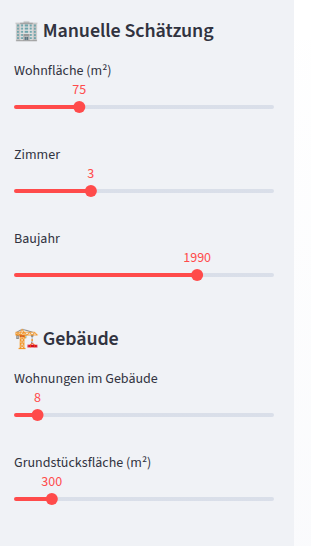
\includegraphics[width=\linewidth]{fig/2026-05-19_13h23_45.png}%
        }{%
            \figplaceholder{6cm}{Manual-input sidebar 1/2 missing.}
        }
    \end{minipage}
    \hfill
    \begin{minipage}[t]{0.42\linewidth}
        \centering
        \IfFileExists{fig/2026-05-19_13h23_59.png}{%
            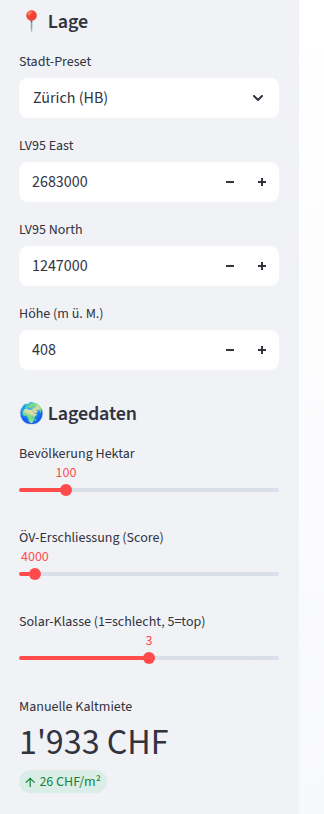
\includegraphics[width=\linewidth]{fig/2026-05-19_13h23_59.png}%
        }{%
            \figplaceholder{6cm}{Manual-input sidebar 2/2 missing.}
        }
    \end{minipage}
    \caption{\textbf{Manuelle Eingabe (fallback).} Left: structural inputs --- Wohnfläche, Zimmerzahl, Baujahr, Wohnungen im Gebäude, Grundstücksfläche. Right: location inputs --- Stadt-Preset (Zürich, Bern, Basel, Genf, $\ldots$), LV95 East/North, Höhe, Bevölkerung im Hektar, ÖV-Erschliessungs-Score, Solar-Klasse. Switching the Stadt-Preset pre-fills the coordinates and the population/ÖV defaults, so a user can quickly explore ``what would this apartment cost in another city?''. The live estimate updates instantly on every slider change.}
    \label{fig:app-manual}
\end{figure}

% =========================================================
\section{Conclusions}
\label{sec:conclusions}

\paragraph{Summary.}
The project produced a reproducible regression pipeline for Swiss apartment cold rents. It starts at the custom \texttt{rentumo.ch} scraper, runs through enrichment with GWR and swisstopo data, and ends with feature engineering, model training and a structured evaluation. The strongest model in the comparison is a LightGBM regressor that uses the KNN-distance features. On the evaluation split it reaches an RMSE of 393~CHF and an R$^2$ of 0.751, which improves on the mid-term mean-prediction baseline of 847~CHF by more than half. The original hypothesis, that a tree-based model outperforms linear regression on this dataset, is therefore clearly supported.

\paragraph{Limitations.}
\begin{itemize}
    \item \textbf{Snapshot dataset.} Only one extraction date (13.04.2026). The model cannot react to market trends.
    \item \textbf{Coverage bias.} Urban areas are over-represented; small-town and rural listings are under-represented.
    \item \textbf{Expensive-apartment error.} The model is roughly twice as inaccurate for the top-quartile apartments. The available structural features do not capture luxury attributes (view, finish, floor).
    \item \textbf{Single platform.} All listings come from rentumo.ch. Comparis was explicitly excluded after written notice.
    \item \textbf{No deployment.} The Streamlit demo runs locally only; production hosting is out of scope for DSPRO1.
\end{itemize}

\paragraph{Future work.}
A few concrete next steps would have the highest impact:

\begin{enumerate}
    \item Extract text-based features from the listing descriptions. Attributes such as balcony, parking spot, renovation year, floor level or lake view are likely the missing piece for the expensive apartments, since the current tabular fields do not capture them.
    \item Pull listings from a second rental platform, for example homegate.ch or immoscout24.ch. This would reduce the urban coverage bias and roughly double the training set.
    \item Replace single-point predictions with prediction intervals using conformal prediction (for example via MAPIE). The demo app could then display estimates as ``CHF $X \pm Y$'' instead of a single number.
    \item Move the demo from a local Streamlit instance to a small hosted application on Streamlit Cloud or Render. This is a natural first deliverable for DSPRO2.
\end{enumerate}

% =========================================================
\section{References}
\label{sec:references}

\bibliographystyle{plainnat}
\bibliography{references}

\end{document}
